\documentclass[5p]{elsarticle}

\usepackage{color}
\usepackage{graphicx}
\usepackage{amssymb}
\usepackage{lineno}
\usepackage{url}
\usepackage{bm}
\journal{Journal Name}
\begin{document}
\begin{frontmatter}
\title{Hierarchical Bayesian inversion of evoked N20 somatosensory current distribution in E/MEG with finite element modeling}
%\title{Applied Inversion Approach of Hierarchical Bayesian Reconstruction for Detecting the Evoked N20 Somatosensory Current Distribution in E/MEG Data
%Hierarchical Bayesian Inversion of the Somatosensory Evoked N20 component in EEG and MEG using a Finite Element head model  

\author[ADD1]{Atena Rezaei}
\author[ADD1,ADD2]{Qin He}
\author[ADD1,ADD4]{Alexandra Koulouri}
\author[ADD1,ADD5]{Ville Rimpil\"{a}inen}
\author[ADD3]{Carsten H.\ Wolters}
\author[ADD1]{Sampsa Pursiainen}
\address[ADD1]{Laboratory of Mathematics, Tampere University of Technology, P.O.\ Box 692, 33101 Tampere, Finland}
\address[ADD2]{Laboratory of Signal Processing, Tampere University of Technology, Tampere, Finland, P.O.\ Box 553, 33101 Tampere, Finland}
\address[ADD4]{Department of Physics, Aristotle University of Thessaloniki, Thessaloniki 541 24, Greece}
\address[ADD5]{Department of Physics, University of Bath, Claverton Down, BA2 7AY Bath, United Kingdom}
\address[ADD3]{Institute for Biomagnetism and Biosignalanalysis, University of M\"{u}nster, Germany, Malmedyweg 15, D-48149 M\"{u}nster, Germany} 

\begin{abstract}
This paper concentrates on advancing computational inversion methods in Elect\-ro-/Mag\-ne\-to\-ence\-phalo\-graphy (E/MEG) in which the neural activity of the brain is detected through non-invasive sensing of the electric/magnetic field surrounding the brain.
\textcolor{red}{ This paper concentrates on advancing computational inversion methods where the neural activity of the brain is detected through non-invasive sensing using Elect\-ro- (EEG) and Mag\-ne\-to\-ence\-phalo\-graphy (MEG).}

We investigate a hierarchical Bayesian approach, concentrating on the detection of the N20 component of evoked human somatosensory activity via clinical E/MEG data and a magnetic resonance imaging (MRI) based multi-compartment head segmentation. \textcolor{red}{We investigate a hierarchical Bayesian approach for the reconstruction of the sources underlying the N20 component of human somatosensory evoked potential (SEP) and field (SEF) activity.} As the forward model, we apply a finite element method (FEM) discretization of a realistically-shaped six compartment head volume conductor and model the neural activity as a current preserving vector field in the grey matter compartment. In our experiments, the present inversion approach was found to be sufficient for distinguishing primary currents at the cytoarchitectonic area 3b  in the posterior wall of the central sulcus. Conditional mean (CM) estimation via Markov chain Monte Carlo (MCMC) sampling was found to improve the source distinction in the deep part of the area 3b as compared to {\em maximum a posteriori} (MAP) optimization  results. The finite element mesh accuracy and the choice for the hyperprior were found to affect on the quality of the inversion outcome. The present results were obtained using the {\em Zeffiro Forward and Inverse Interface for EEG/MEG Imaging} which is an accessible and simple-to-use open-source software tool utilizing the Matlab programming environment.
\end{abstract}

\begin{keyword}
\texttt{Electroencephalography (EEG)}\sep
\texttt{Magnetoencephalography (MEG)}\sep
\texttt{Evoked Somatosensory Activity}\sep
\texttt{Finite Element Method (FEM)}\sep
\texttt{Iterative Alternating Sequential}\sep
\texttt{Bayesian Method}\sep
\texttt{Clinical Data}
\end{keyword}

\end{frontmatter}

%\linenumber

%% main text
\section{Introduction}
\label{S:1}

This paper investigates computational inversion methods in Electro-/Magneto\-en\-cephalo\-graphy (E/MEG) \cite{hamalainen1993,niedermeyer2004} detection of median nerve stimulation together with a magnetic resonance imaging (MRI) based multi-compartment head segmentation. Our goal is to distinguish the N20 response of the stimulus in the cytoarchitectonic Brodmann area 3b \cite{haueisen2007identifying,buchner1994source,hari2018ifcn,baumgartner2010dipole} which is located in the posterior wall of the central sulcus (Figure \ref{fig:somatosensory_cortex}). We reconstruct the primary current field of the neurons as a three-dimensional distribution restricted to the grey matter of the brain. This is an ill-conditioned inverse problem in which the applied prior model and reconstruction technique have a major effect on  the final result \cite{brette2012}. That is the reason why {\em prior} information such as clinical neurophysiological knowledge is required. In this case, finding the activity on the sulcus wall is particularly challenging since E/MEG is classically known to be more sensitive to the superficial parts than to the deeper lying areas in the sulci.
%MEG is more sensitive to superficial area than EEG.h
Generally, EEG \cite{ahlfors2010sensitivity} is more sensitive to all types of source orientations, both radial and tangential, while MEG finds more superficial currents in cortical regions. Furthermore, EEG is more sensitive to detecting signal from deeper parts of the brain \cite{hari2018ifcn}.

We reconstruct the activity using the hierarchical Bayesian inversion approach which has been previously shown to be well-suited for reconstructing deep lying activity \citep{calvetti2009,lucka2012,calvetti2018,calvetti2015}.   Bayesian inversion \citep{kaipio2004,calvetti2007,baillet1997bayesian,trujillo2004bayesian,schmidt1999bayesian} enables incorporating the {\em a priori} information of the noise and the uncertainty of the unknown into a single posterior probability density  which can be explored numerically to find a reconstruction. The advantages of this approach are that all kinds of uncertainties, e.g., primary and latent unknowns, can be precisely modeled and that, once formed, the same distribution can be explored with various techniques in order to maximize the knowledge of the unknown. 

The present hierarchical prior model \citep{ohagan2004,calvetti2009,lucka2012} is conditionally Gaussian which allows for adjusting the probability of outliers, i.e., focal sources, via hyperparameters of a gamma and/or inverse gamma hyperprior distribution to estimate a primary current distribution under the uncertainty assumptions. We explore the posterior via both {\em maximum a posteriori} (MAP) optimization and Markov chain Monte Carlo (MCMC) sampling \citep{gelman1995bayesian,liu2001}. In the first one of these, we use the iterative alternating sequential (IAS) technique and in the second one the well-known Gibbs sampler restricted into a spherical region of interest which is chosen based on the MAP estimation results and the neurophysiological {\em a priori} knowledge of the expected neural response. 

As the forward modeling technique \citep{demunck2012}, we apply the finite element method (FEM) \cite{braess2001,CHW:Hau2002,CHW:Ram2006}
which allows for creating an accurate volumetric discretization of a multi-compartment head segmentation  regarding its conductivity distribution and strongly folded tissue structures. The FEM enables placing the neural activity to the grey matter, where it can be aligned in the direction of the inward surface normal corresponding to the orientation of the apical dendrites of the 
pyramidal cells (Figure \ref{fig:somatosensory_cortex}) \citep{creutzfeldt1962influence,hari2018ifcn,hallez2007review}. 



As the source model, we employ the mathematically rigorous current preserving (divergence conforming) H(div) approach which has been introduced and studied for linear (Whitney) basis functions in \citep{bauer2015} and for the general quadratic basis in \citep{pursiainen2016}. In these studies, this approach has been shown to be both a focal and accurate compared to other direct source modeling methods, meaning that it is widely applicable in realistic E/MEG forward simulation \citep{vorwerk2014guideline} which necessitates robustness in the thin and geometrically complex structure of the grey matter compartment \citep{griffis2016age,mcginnis2011age,fischl2000measuring}. 

In the numerical experiments, the present inversion approach was found to be sufficient for distinguishing primary currents in the Brodmann area 3b \citep{brodmann1909vergleichende}  of the primary somatosensory cortex which is constituted by areas 1, 2 and 3 as sketched in Figure \ref{fig:somatosensory_cortex}. The  Gibbs sampler \cite{elliott1984application} was found to improve the source distinction in the deep part of the area 3b as compared to IAS optimization results. The choice for the hypermodel and the finite element (FE) mesh resolution were found to affect on the quality of the inversion estimates. The present results were obtained using the  {\em Zeffiro Forward and Inverse Interface for EEG/MEG Imaging} \cite{ZeffiroInterface} (ZI) which is an accessible and simple-to-use open source software tool utilizing the Matlab (the Mathworks Inc.) programming environment.

\begin{figure}[h!]
\begin{footnotesize}
\begin{center}
\begin{minipage}{7cm} \begin{center}

\includegraphics[width=4.5cm]{area_3b.png}
\end{center}\end{minipage} \vskip0.2cm
\begin{minipage}{7cm} \begin{center}

\includegraphics[width=4.5cm]{normal_currents.png} 
\end{center}
\end{minipage} 
\end{center}
\end{footnotesize}
\caption{{\bf Top:} A schematic picture of the sagittal cut of the primary somatosensory cortex. The N20 component of the somatosensory activity takes place in the Brodmann area 3b which is located in the posterior wall of the central sulcus. {\bf Bottom:} A schematic visualization of the direction of the primary currents of the pyramidal cells which are aligned along the inward surface normal in the cortex.  }
\label{fig:somatosensory_cortex} 
\end{figure}

\section{Methods}

\subsection{Forward model}

The present current preserving H(div) forward model \citep{pursiainen2016}  follows mathematically from the physical condition that the current distribution in the computation domain does not contain local (monopolar) sources or sinks. Consequently, the divergence of the total current, the sum of the primary current (neural activity) and the evoked volume current must be zero, i.e., $\vec{J}^T = \vec{J}^P - \sigma \nabla u$ everywhere. This condition implies the governing quasi-static second order partial differential equation for the electric potential field, i.e.,  \begin{equation} \nabla \cdot (\sigma \nabla u) = \nabla \cdot \vec{J}^P. \end{equation} The current preserving boundary condition ensures that there is no flow into or out of the domain. That is, the normal component of the volume current is zero, i.e., $(\sigma \nabla u) \cdot \vec{n} = 0$, on $\partial \Omega$. https://preview.overleaf.com/public/nscdbdnqmyvg/images/712fa5ac10bf031d91692ef0f68e4082daa3bd37.jpeg

The governing equation can be integrated by parts, if multiplied with a test function $v$ belonging to the Sobolev space $H^1 (\Omega)$, whose members have  square integrable first-order partial derivatives. This results in the weak form $\int_{\Omega} \nabla v \cdot (\sigma \nabla u) dV = - \int_{\Omega} v ( \nabla \cdot \vec{J}^P ) \,  dV$ which must be satisfied for all $v \in H^1 (\Omega)$. The weak form uniquely solvable up to choosing the ground level \citep{evans1998, CHW:Dre2009}, if the divergence of the primary current density has a finite energy, i.e., if it belongs to the space $\vec{J}^P \in H(\hbox{div}) = \{\vec{w} | \nabla \cdot \vec{w} \in L^2 (\Omega) \}$ of functions with square integrable divergence.  

In the classical Ritz-Galerkin FE discretization of $\Omega$ \citep{braess2001}, $u$ and $\vec{J}^P$ are approximated as the  finite sums $u_h = \sum_{i=1}^N z_i \psi_i$ and $\vec{J}_{h}^P = \sum_{j=1}^K x_j \vec{w}_j$, where  $\psi_1, \psi_2, \dots, \psi_N \in H^1(\Omega)$ and   $\vec{w}_1, \vec{w}_2, \dots , \vec{w}_K \in H(\hbox{div})$ are  piecewise linear (nodal) scalar valued and divergence conforming vector valued FE basis functions, respectively \citep{pursiainen2016}.  Associating $u_h$ and $\vec{J}_{h}^P$ with coordinate vectors $\mathbf{z} = ( z_1, z_2, \dots, z_N )$ and $\mathbf{x} = (x_1, x_2, \dots , x_K)$, the weak form turns into a linear system of equations $\mathbf{Az} = \mathbf{Gx}$ where $\mathbf{A} \in \mathbb{R}^{(N \times N)}$  and $\mathbf{G} \in \mathbb{R}^{(N \times K)}$ with $A_{i,j}=\int_{\Omega} \nabla \psi_j \cdot ( \sigma \nabla \psi_i )dV$ and $G_{i,j} = \int_{\Omega} \psi_i (\nabla \cdot \vec{w}_j)dV$. The solution unique if, additionally, the ground level is specified, for example, by associating one of the degrees of freedom with the ground. 

The eventual E/MEG forward model is predicted by the lead field equation ${\bf y} = {\bf L} {\bf x}$ where the lead field matrix is of the form ${\bf L} = {\bf R} {\bf A}^{-1} {\bf G} $ for EEG with ${\bf R}$ denoting a restriction matrix which picks the electrode potential field values at the measurement points. Technically, the lead field matrix can be obtained by evaluating the transfer matrix ${\bf T} = {\bf A}^{-1} {\bf R}^t$ .  The MEG lead field matrix and its transfer matrix can be obtained via a similar procedure based on the Biot-Savart formula in which which the total current field is integrated over the domain \citep{pursiainen2012,sato2004hierarchical}. 

\subsection{Hierarchical Bayesian model}

For a single given data set ${\bf y}$, the classical Bayes formula for subjective conditional probabilities can be written as
\begin{equation}
p ( {\bf x} \mid {\bf y})  =   \frac{p({\bf x}) \, p({\bf y} \mid {\bf x})} {p({\bf y})} \propto  {p({\bf x}) \, p({\bf y} \mid {\bf x})}.  
\end{equation} 
That is, the {\em posterior} probability density $p({\bf x} \mid {\bf y})$ of the  unknown primary current distribution ${\bf x}$ in the brain is proportional to the product between the prior density $p({\bf x})$, i.e., the {\em a priori} knowledge of ${\bf x}$, and the likelihood function $p({\bf y} \mid {\bf x})$ following from the measurement noise model \cite{schmidt1999bayesian}. 

Here, the measurement error is assumed to be a Gaussian zero mean random vector ${\bf n} = {\bf y} - {\bf L} {\bf x}$ with independent entries, i.e., the likelihood is of the form  $p({\bf y} \mid {\bf x}) \propto \exp ( - (2  \sigma^2)^{-1} \| {\bf L} {\bf x} - {\bf y}\|^2 )$, where $\sigma$ is the standard deviation of the noise. Furthermore, it is assumed that the prior is a joint density 
\begin{equation}
p ( {\bf x}, {\bf h}) \propto  p({\bm \theta}) \,  p ( {\bf x} \mid {\bm \theta})
\end{equation}
of ${\bf x}$ and a hyperparameter ${\bm \theta}$, meaning that the actual prior is, in fact, a marginal density of the form 
\begin{equation}
p ( {\bf x}) \propto  \int p({\bm \theta}) \,  p ( {\bf x} \mid {\bm \theta}) \, \hbox{d} {\bm \theta}. 
\end{equation}                                                                                                                                                                                        
The conditional part $p ( {\bf x} \mid {\bm \theta})$ is also a zero mean Gaussian density. Its diagonal covariance matrix is predicted by a long-tailed hyperprior $p ({\bm \theta})$, meaning that the variance vector, i.e., the set of diagonal entries, is likely to contain outliers. Consequently, it is implicitly assumed that ${\bf x}$ is a sparse vector, i.e., it has a small set of entries which are considerably larger in absolute value than the others \cite{sato2004hierarchical}. The number and intensity of these outliers are controlled by the hyperprior \cite{calvetti2007gaussian}. This impulse-like prior model for the unknown is  advantageous since the goal in the inversion is to obtain a focal reconstruction for the brain activity, meaning that only a small part of the entries in ${\bf x}$ differ essentially from zero. As the hyperprior, we test both the gamma $\hbox{G}({\bm \theta} \mid \beta, \theta_0)$ and inverse gamma $\hbox{IG}({\bm \theta} \mid \beta, \theta_0)$ distribution whose density  is supported on the set of non-negative real numbers with a structure determined by the scale  and shape parameter $\theta_0$ and $\beta$, respectively. The first one of these controls the effective size of the support as well as the distance of the maximum from the origin, the greater value the larger support and greater maximum. Again, the second one steers the decay rate of the tail. 

We use an approach in which, instead of marginalization, $\beta \geq 1.5$ and $\theta_0 > 0$ are subjectively chosen by the scientist. The scale parameter $\theta_0$ can here be interpreted as the sensitivity of the prior. The sensitivity to detect activity  grows along with the value of $\theta_0$. A lower sensitivity means a more focal reconstruction (less non-zero entries in ${\bf x}$) but also a higher vulnerability to noise effects and numerical estimation errors. Namely, the posterior density for a very low  value of $\theta_0$ will be very concentrated around a certain region which can be difficult to be found numerically, when exploring the posterior. In such a situation, to ease up the reconstruction process, one can increase the value of the shape parameter $\beta$ which should, nevertheless, be as small as possible in order to optimize the focality of the reconstruction.  

Given the posterior, the actual reconstruction can be found via several different approaches. The most common ones can be divided to optimization and sampling techniques. The former ones, e.g., the {\em maximum a posteriori} (MAP) algorithms, which maximize the posterior density, i.e., 
$ x_{MAP} = \hbox{argmax } p_{\hbox{\scriptsize post}}(x, \theta\mid y)$
for $x\in\mathbb{R}^k$ \cite{lucka2012} usually provide the faster way but less robust way to obtain a reconstruction than the sampling techniques which, on one hand, are computationally expensive but, on the other hand, constitute a reliable alternative for finding a numerical estimate representing the global structure of the posterior, e.g., the conditional mean (CM) which can be denoted as $x_{CM} = E(x,\theta\mid y)= \int (x,\theta)p_{\hbox{\scriptsize post}}(x,\theta \mid y) \, \hbox{d} x \hbox{d} \theta$ \cite{calvetti2009}. In general, CM is more robust and MAP is more sensitive to noise than the center of probability mass.

\subsection{Iterative alternating sequential MAP estimation}

As a MAP estimation technique, to estimate the optimal unknown parameter, we use the iterative alternating sequential (IAS) algorithm \citep{calvetti2007gaussian,calvetti2008hypermodels}
which was introduced for E/MEG in \cite{calvetti2009}. IAS is effectively a steepest descent method which  alternates between the ${\bf x}$ and ${\bm \theta}$ component in the set of candidate solutions. The algorithm can be expressed as follows: 
\begin{enumerate} 
\item Set $k = 1$ and ${\bm \theta}^{(1)} = (\theta_0, \theta_0, \ldots, \theta_0)$ as the initial prior variance. Choose the desired number  of iteration steps $K$. 

\item Find the maximizer ${\bf x}^{(k)}$ of the conditional posterior $p ({\bf x} \mid {\bf y}, {\bm \theta}^{(k)})$.
\item Find the maximizer ${\bm \theta}^{(k+1)}$ of the conditional posterior $p ({\bm \theta} \mid {\bf y}, {\bf x}^{(k)})$.
\item Set $k \to k + 1$. If $k < K$, repeat the second and third step. 
\end{enumerate}
The IAS iteration usually converges in a relative low number of iteration steps, e.g., three. The method is computationally advantageous, firstly, as the second step can be performed via solving a linear system of equations in which the size of the governing square matrix matches with the length of the data vector, i.e., it is relatively small. Secondly, the third step can be achieved explicitly through a straightforward substitution into a formula determining the zero point of the derivative of $p ({\bm \theta} \mid {\bf y}, {\bf x}^{(k)})$. Furthermore, for the gamma hyperprior, if $\beta = 1.5$, the estimate found by the IAS iteration has been shown  to coincide with the {\em minimum current estimate}, i.e., the $\ell^1$-regularized solution of the inverse problem \cite{uuhaso99,hauk2004keep,auranen2005}. Again, for the inverse gamma hyperprior, there is a correspondence to the {\em minimum support estimate}    \citep{calvetti2009}.

\subsection{Gibbs sampler}

We estimate the CM using the {\em Gibbs sampler}, a well-known {\em Markov chain Monte Carlo} (MCMC) sampling technique \cite{kaipio2004} which estimates the source currents randomly over a lattice of points  \cite{spitzer1971markov} by sampling each component with respect to the previous values of other variables \cite{murphy2012machine}. The algorithm draws random from one-dimensional conditional densities proceeding as follows:
\begin{enumerate}
\item Set k = 1. Choose the desired sample size $K$ and set ${\bf x}^{(1)} = (0, 0, \ldots, 0)$. 
%\item For $i = 1, 2, \ldots, n$, draw a random number ${t}^\ast$ from the one-dimensional conditional density \[ p(t \mid z_1, \ldots, z_{i-1}, x^{(k)}_{i+1}, \ldots, x^{(k)}_n, {\bm \theta}^{(k)}) \] and set $z_i = t^\ast$.
\item For $i = 1, 2, \ldots, n$, draw a random vector ${\bf z}$ from the conditionally Gaussian density $p({\bf x} \mid {\bf y}, {\bm \theta}^{(k)})$ applying an affine transform to a random realization of Gaussian white noise as shown in \cite{calvetti2009}. 
\item For $i = 1, 2, \ldots, n$, draw a random number ${t}^\ast$ from the one-dimensional conditional density \[ p(t \mid {\bf y}, \zeta_1, \ldots, \zeta_{i-1}, \theta^{(k)}_{i+1}, \ldots, \theta^{(k)}_n, {\bf x}^{(k+1)}) \] and set $z_i = t^\ast$.
\item Set ${\bf x}^{(k+1)} = {\bf z}$, ${\bm \theta}^{(k+1)}  = (\zeta_1, \zeta_2, \ldots, \zeta_n)$  and $k \to k + 1$. If $k < K$, repeat the second and third step. 
\end{enumerate}

The one-dimensional draw of the third step requires finding the interval in which the posterior density is supported and evaluating it in a suitably chosen set of points over the interval. For a large $n$, the sampling process can be slow and computationally expensive, as a relatively large number of sampling points has to be created for the posterior which has an unknown structure and, moreover, as one needs to operate with the large lead field matrix each time the posterior is evaluated. Consequently, we limit the sampling in a small ($n <<N$) region of interest (ROI) which was, in this study, a 24 mm diameter ball chosen based on the neurophysiological {\em a priori} knowledge of the evoked somatosensory N20 activity and also on preliminary MAP estimation tests.  

\subsection{Numerical Model} 

\subsubsection{Head segmentation}

\begin{figure}[h!]
\begin{footnotesize}
\begin{center}
\begin{minipage}{3.8cm} \begin{center}
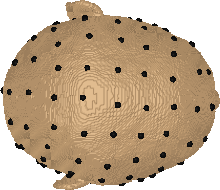
\includegraphics[height=2.6cm]{electrodes.png} 
\end{center}\end{minipage}
\begin{minipage}{3.8cm} \begin{center}
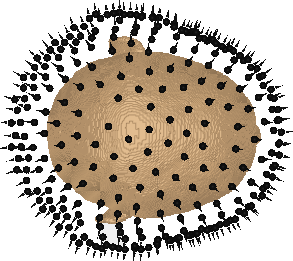
\includegraphics[height=3.6cm]{magnetometers.png}
\end{center}\end{minipage} \\ \mbox{} \vskip0.2cm \mbox{} 
\begin{minipage}{3.8cm} \begin{center}
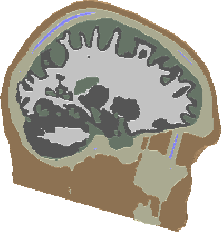
\includegraphics[height=3.0cm]{1mm_mesh.png} 
\end{center}\end{minipage} 
\begin{minipage}{3.8cm} \begin{center}
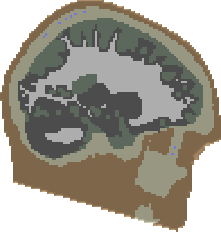
\includegraphics[height=3.0cm]{2mm_mesh.png} 
\end{center}\end{minipage} 
\end{center}
\end{footnotesize}
\caption{{\bf Top row:} A top view of the positions for the successfully recorded 72 electrode (left) and 271 magnetometer (right)   channels. The magnetometer orientations are also shown. {\bf Bottom row:}  A sagittal cut of the six compartment tetrahedral FE mesh for 1 and 2 mm resolution (left and right, respectively). The modeled compartments are the following: skin (brown), compact bone (beige), spongious bone (blue), cerebrospinal fluid (green), grey matter (grey) and white matter (light grey). Comparing the two different meshes it is obvious that the 1 mm resolution is essential for the physiological accuracy of the volume conductor model, for example, based on the non-connected spongious compartment and missing white matter structures in the 2 mm mesh.  }
\label{fig:head_model} 
\end{figure}

In this study, the principal FE implementation approach presented in \citep{pursiainen2012} was applied including the formulas for the E/MEG lead field matrices: a tetrahedral finite element mesh for $\Omega$ was generated by subdividing each voxel in a surface based regular hexahedral segmentation into six tetrahedra.

The FE meshes were generated using a six-layer surface segmentation created using T1-weighted and T2-weighted MRI sequences recorded with a 3 T MRI scanner. The surfaces (level-sets) of  skin, compact bone (skull), spongious bone (skull), cerebrospinal fluid (CSF), grey matter and white matter were included in the model.  The surfaces were distinguished using various methods as described in \cite{nusing2018}. A FE mesh was generated for both 1 and 2 mm resolution (voxel size). The first one of these included 3.8 M nodes and 22 M tetrahedra and the second one 0.47 M nodes and 2.7 M tetrahedra. A sagittal cut of each mesh is illustrated in Figure \ref{fig:head_model}.

\subsubsection{Source space}

As the source space, we used the  quadratic H(div) approach presented in \citep{pursiainen2016,miinalainen2019}, employing the {\em Position Based Optimization} (PBO) interpolation with the 10-source (8-point) stencil in which a given dipolar current source is estimated via the 4 linear face and 6 quadratic edge vector basis functions associated with the barycenter of the tetrahedron containing the source position. 

The primary current sources were placed in the interior part of the grey matter compartment in the elements with a full set (four) of neighbors belonging to the same compartment. The rest of the compartment forming the boundary layer of the grey matter contained no sources, since it is known to be less advantageous regarding the modeling accuracy than the interior part \cite{miinalainen2019}.

To obtain an uniform (mesh independent) source density, 100000 points were   distributed randomly in the grey matter for each FE mesh. A uniform point spread was obtained through a straightforward random permutation due to the uniform mesh structure. The points placed on the boundary layer in the initial stage were filtered out of the eventual distribution consisting of 76000 and 61000 positions for 1 and 2 mm resolution, respectively. The lower source count for the 2 mm case was caused by the thicker boundary layer following from the larger element size.   Each position comprised three sources oriented along the three Cartesian coordinate axes. Hence, the total number of sources was 228000 and 183000 for 1 and 2 mm, respectively.

The Cartesian set of sources was used in inverting the data. The results were then visualized applying the neurophysiological normal constraint (Figure \ref{fig:somatosensory_cortex}), by showing the reconstructed activity pointing in the direction of the inward surface normal. 

\subsubsection{Clinical and synthetic data}

\begin{figure}[h!]
\begin{footnotesize}
\begin{center}
\begin{minipage}{4.3cm} \begin{center}
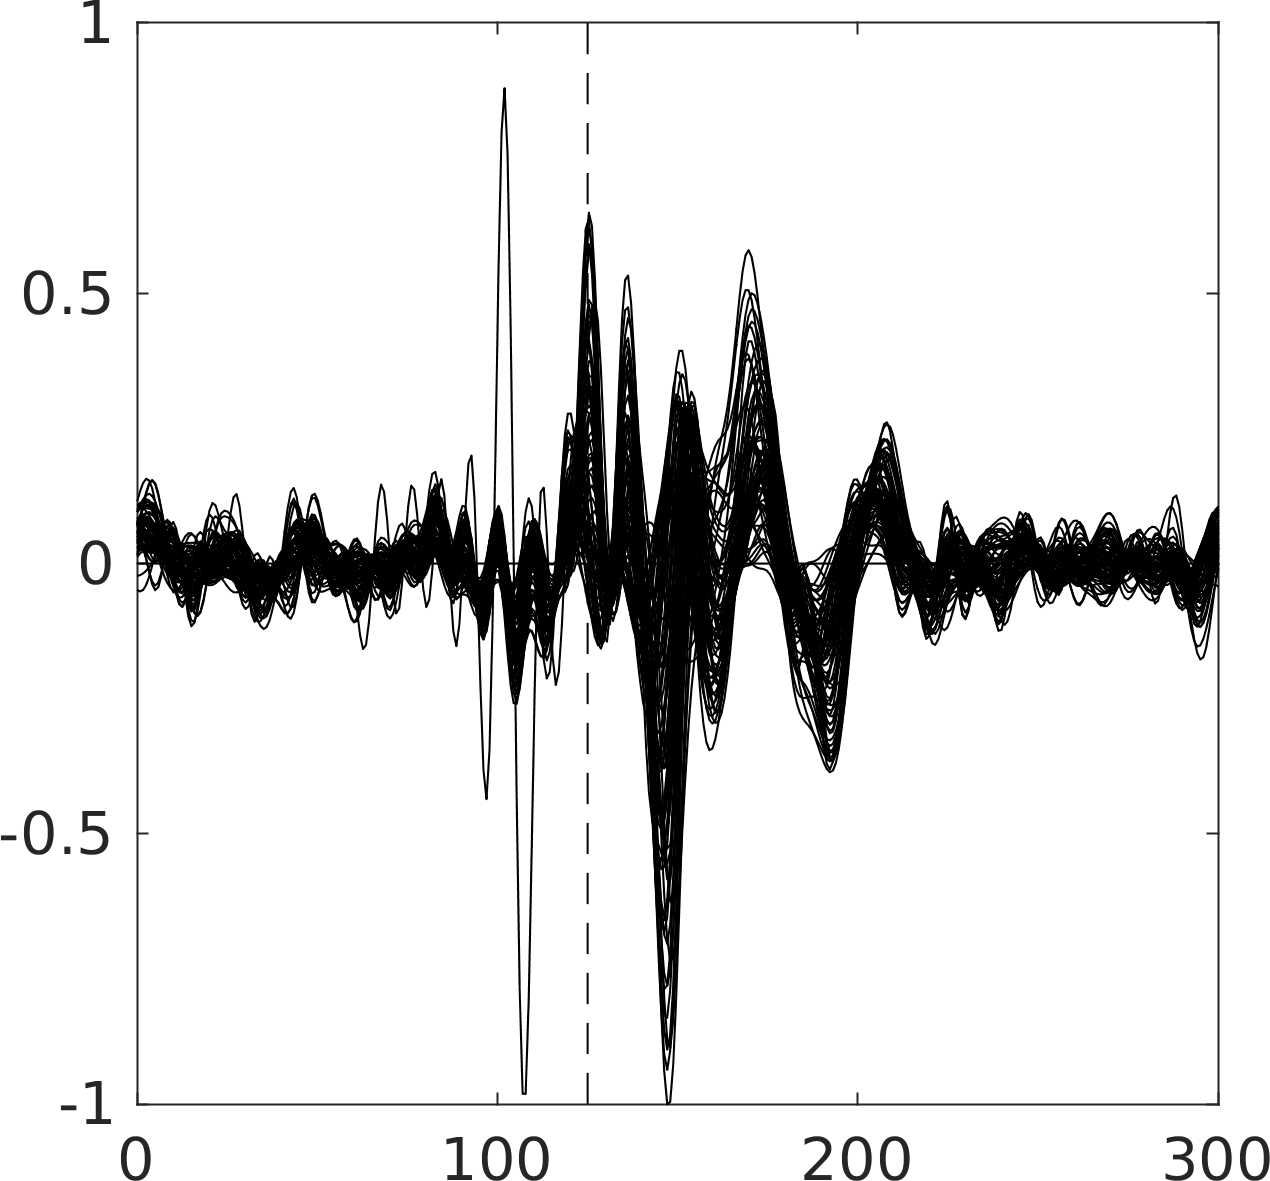
\includegraphics[height=4.1cm]{eeg_data.png} \\ EEG data
\end{center}\end{minipage}
\begin{minipage}{4.3cm} \begin{center}
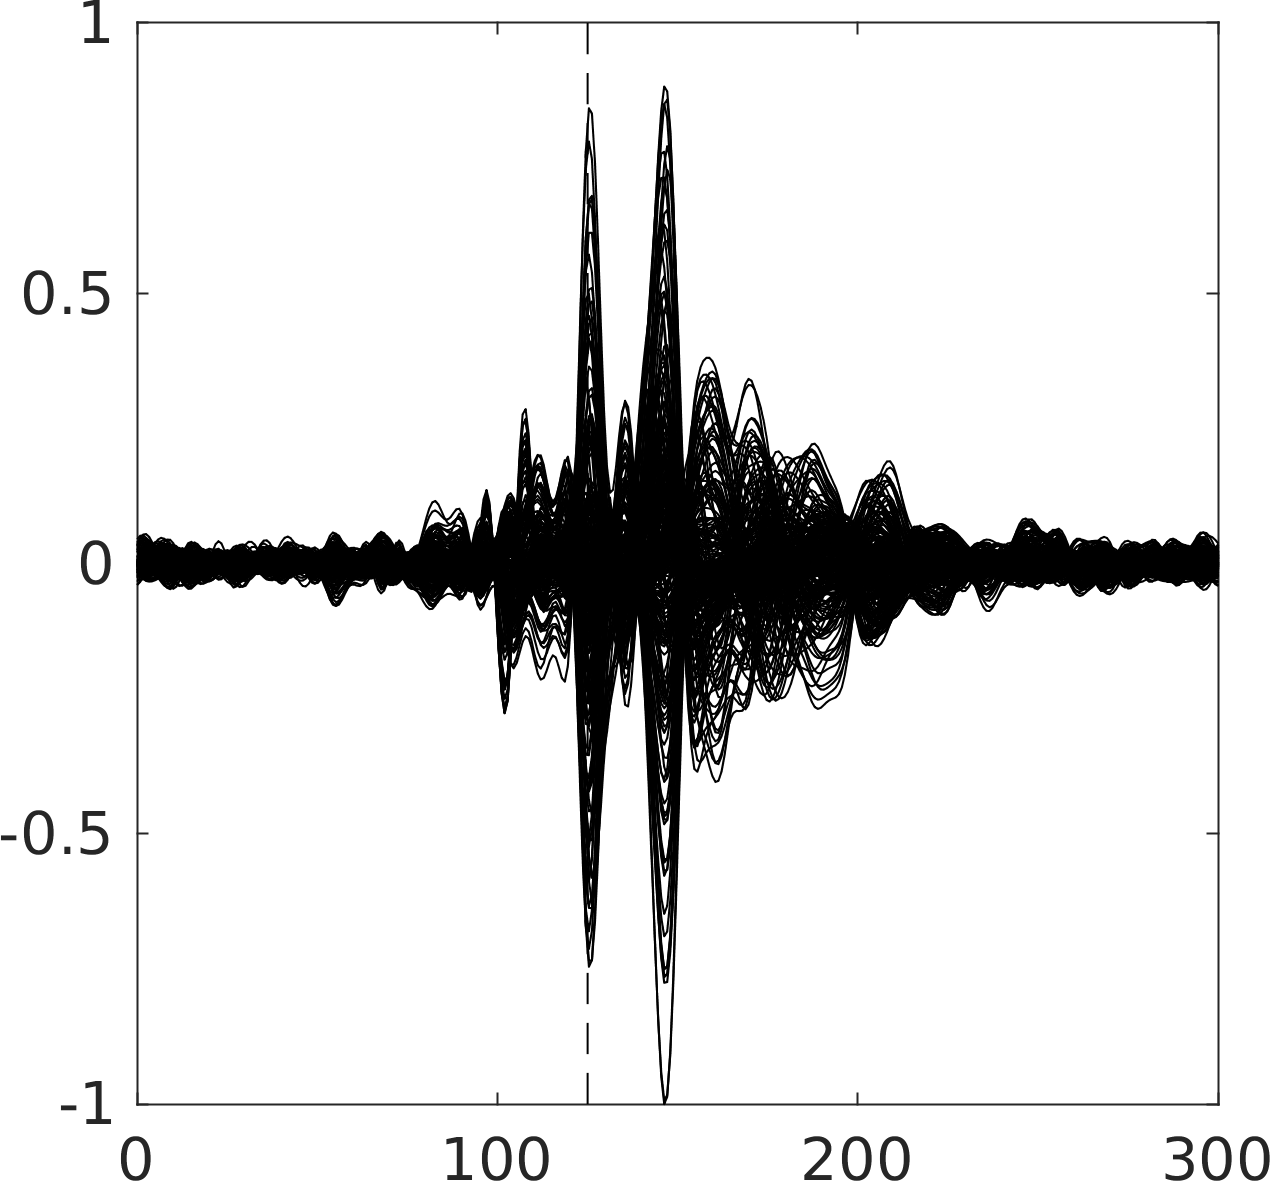
\includegraphics[height=4.1cm]{meg_data.png} \\ MEG data
\end{center}\end{minipage} 
\end{center}
\end{footnotesize}
\caption{The  parallel EEG (left) and MEG (right)  measurements with the amplitude normalized to one.  The actual stimulus response is measured for the interval  100--200 ms which is  preceded and followed by the pre-stimulus and post-stimulus phase, respectively. The N20 component investigated in this study corresponds to the peaks centered at 125 ms total time, that is, 25 ms after the stimulus (vertical dashed line). }
\label{fig:data} 
\end{figure}


The numerical experiments were conducted  using a data set measured during the stimulation of the right median nerve of a right-handed, 49-year-old, male subject lying in a supine position. EEG and MEG data were recorded in parallel successfully for 72 electrodes and 271 magnetometers (Figure \ref{fig:head_model}). The total number of 1200 stimuli were applied. A single stimulus had a 300 ms total duration which was subdivided into 100 ms pre-stimulus, stimulus and post-stimulus subintervals. The inter-stimulus interval varied between 350 and 450 ms. The measurements were pre-processed using a notch filter for the frequency 50 Hz and for its harmonics to remove the power-line noise. The response measured for the different stimuli where averaged to produce the evoked potential data the amplitude of which was normalized to one (Figure \ref{fig:data}).

The eventual signal to be inverted corresponded to the N20 activity occurring at 25 ms in the actual stimulus phase, i.e., at 125 ms total time (Figure \ref{fig:data}). The data vector ${\bf y}$ for the inversion computation, a was obtained by centering at 125 ms a Gaussian window with the length 50 ms and applying a short-time Fourier tranform based  band-pass filter for the frequency interval 20--250 Hz.

In addition to the clinical data, for comparison, a synthetic dipolar source was placed, on the 3b area in the posterior wall of the central sulcus oriented along with its inward normal. The data for the source was estimated using the present FEM forward simulation and additive zero mean Gaussian noise with 3 \% standard deviation with respect to the maximal signal amplitude. The same noise model was used also to obtain the likelihood function for the clinical data.   

\subsubsection{Inverse Estimates}

The details of the inverse estimates computed in this study are included in Table \ref{tab:inverse_estimates}. The hyperparameters were chosen subjectively case-by-case, based on the {\em a priori} knowledge that the reconstruction of the N20 component should be concentrated at or near the 3b area. 
As a general rule, the smaller the scale parameter the deeper activity is shown by the reconstruction. Using a sufficiently small value was necessary in order to avoid overly superficial estimates. On the other hand, a too small value led to  erroneous reconstructions. 

The scale parameter value applied was, in general, smaller for EEG than for MEG. Again, CM computation allowed using a smaller scale parameter than what was possible in MAP estimation. The shape parameter value 1.5 worked well in finding a MAP estimate. In the case of CM, a somewhat larger value was chosen in order to shorten the tail of the reconstruction and, thereby, to avoid overly focal reconstructions (Figure \ref{fig:gamma_vs_inverse_gamma}), which was necessary especially for IG. Each estimate was computed using both real and synthetic data. The number of three IAS iterations in MAP estimation was sufficient. For CM, a sample of 10000 points was created with the Gibbs sampler. Of these, 1000 points in the beginning of the sequence were neglected as a burn-in phase. 

The ROI (Figure \ref{fig:roi}) for the CM sampling was chosen based on preliminary EEG MAP estimation tests. The synthetic source was placed and oriented in the ROI in the posterior  wall of the central sulcus as shown in Figure \ref{fig:source_placement}.

\begin{figure}[h!]
\begin{footnotesize}
\begin{center}
\begin{minipage}{3.9cm} \begin{center}
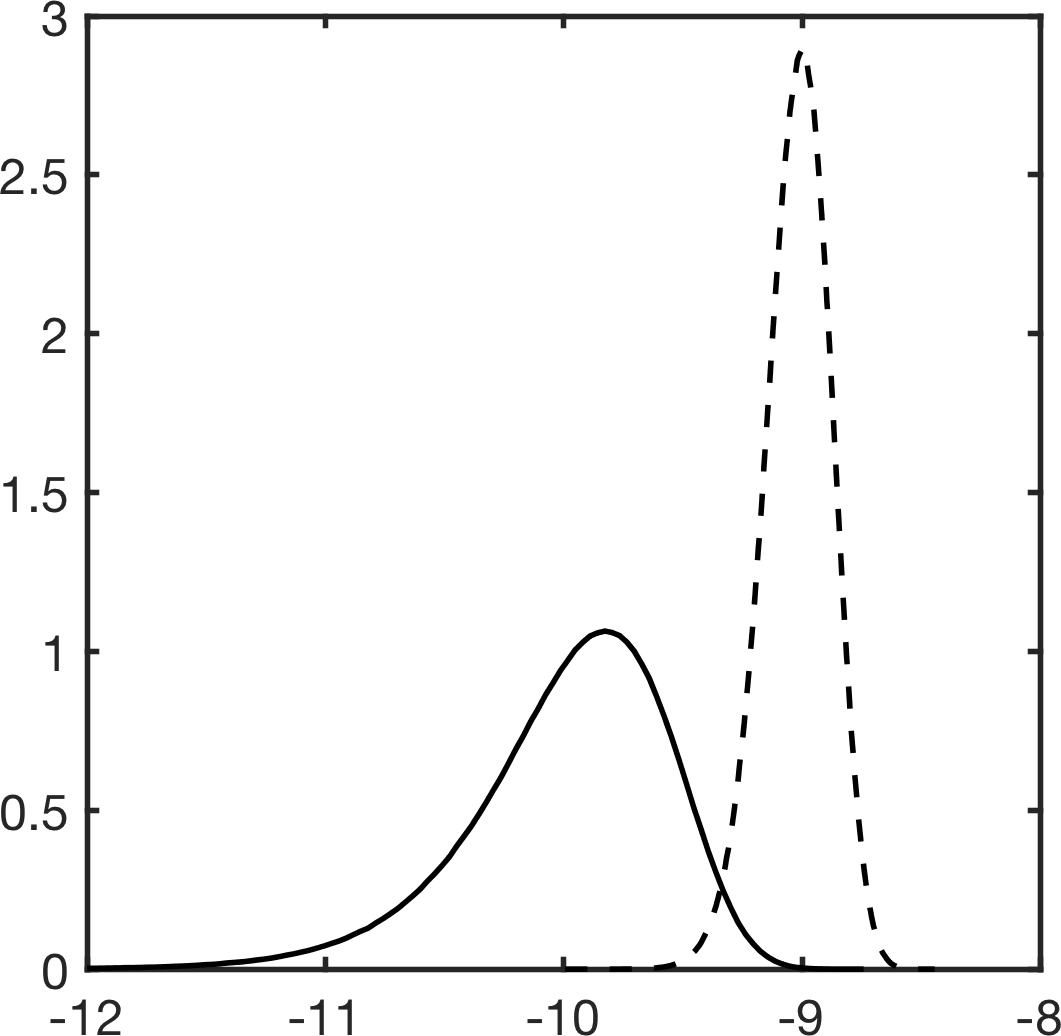
\includegraphics[width=3.5cm]{gamma_density.png} \\ Gamma 
\end{center}\end{minipage} 
\begin{minipage}{3.9cm} \begin{center}
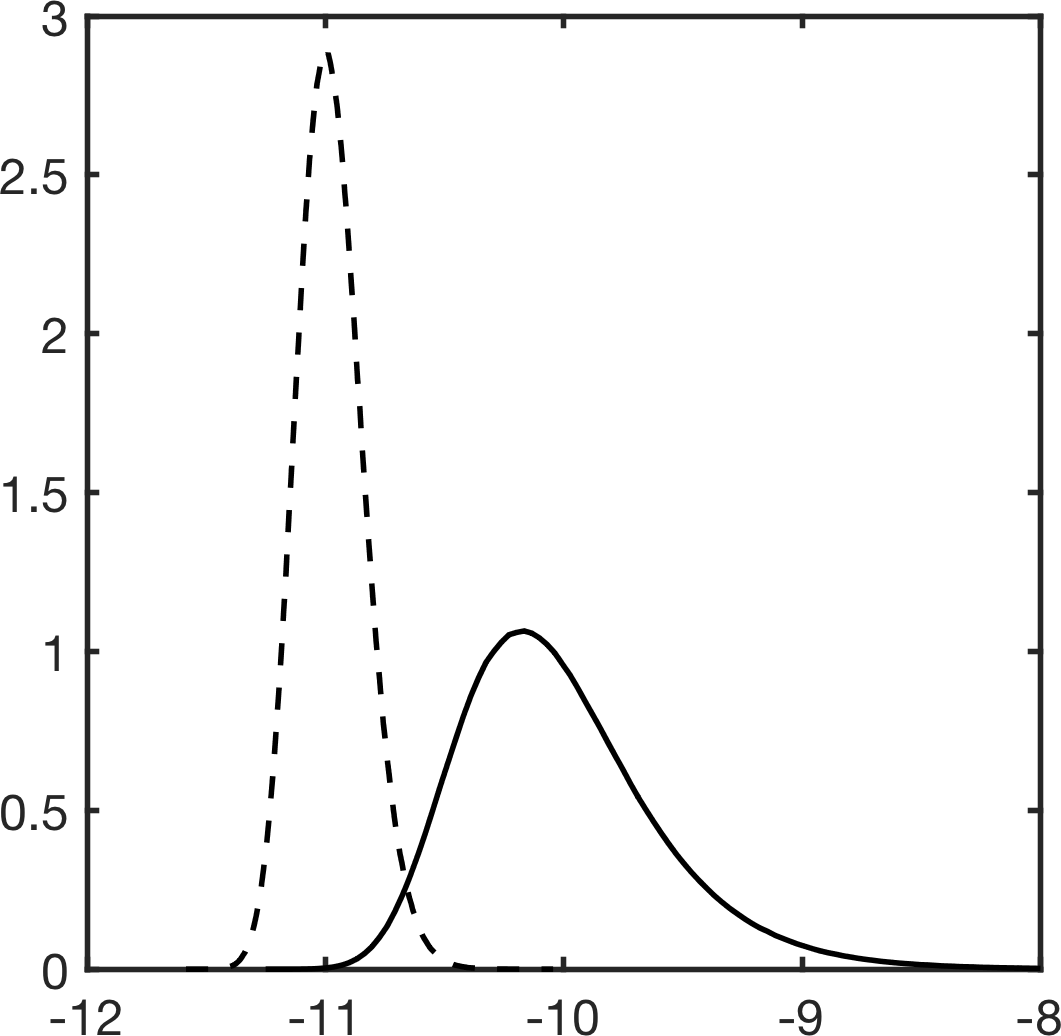
\includegraphics[width=3.5cm]{inverse_gamma_density.png} \\ Inverse gamma
\end{center}
\end{minipage} 
\end{center}
\end{footnotesize}
\caption{An illustration of the gamma (G) and inverse gamma (IG) probability density. The scale of the x-axis is logarithmic with base 10 in order to make the tail part of the density visible. In the direction of the y-axis the scale is linear. In each case, the scale parameter is $\theta_0 = 10^{-10}$. The solid line corresponds to the shape parameter value $\beta = 1.5$ and the dashed one to $\beta = 10$. The smaller $\beta$ the longer the tail.  With equal hyperparameters, IG has a longer tail than G, meaning that the IG hyperprior gives more emphasis on very focal distributions. The maximum of the density increases/decreases along with $\beta$ for G/IG, respectively. }
\label{fig:gamma_vs_inverse_gamma} 
\end{figure}

\begin{figure}[h!]
\begin{footnotesize}
\begin{center}
\begin{minipage}{3.9cm} \begin{center}
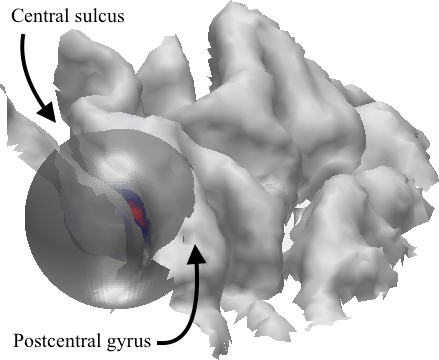
\includegraphics[height=3.8cm]{ROI.png} 
\end{center}\end{minipage}
\end{center}
\end{footnotesize}
\caption{The region of interest (ROI)  utilized in the CM computations is the region restricted by the 24 mm diameter grey spherical surface centralized on the central sulcus of the left hemisphere. The number of A MAP estimate for synthetic EEG data is visualized on the cortex. }
\label{fig:roi} 
\end{figure}

\begin{figure}[h!]
\begin{footnotesize}
\begin{center}
\begin{minipage}{3.8cm} \begin{center}
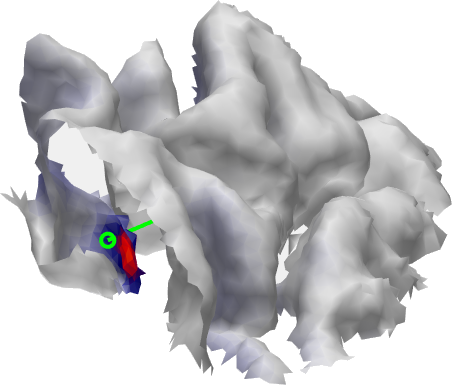
\includegraphics[height=2.7cm]{EEG_source_synthetic_data.png} \\ Synthetic data
\end{center}\end{minipage}
\begin{minipage}{3.8cm} \begin{center}
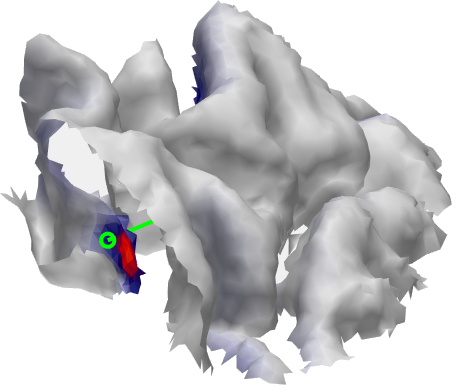
\includegraphics[height=2.7cm]{EEG_source_real_data.png} \\ Clinical data
\end{center}\end{minipage} \begin{minipage}{0.5cm} \begin{center}
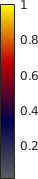
\includegraphics[height=2.7cm]{colorbar.png} \\ \null
\end{center}
\end{minipage} 
% \vskip0.2cm
% \begin{minipage}{3cm} \begin{center}
% 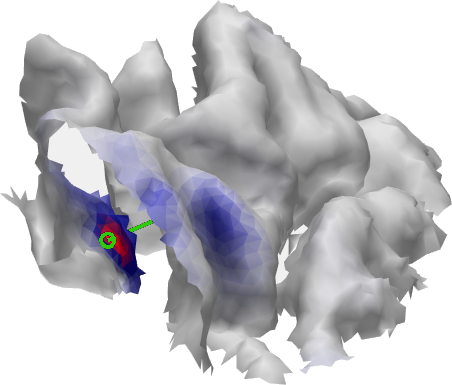
\includegraphics[height=2.0cm]{MEG_source_synthetic_data.png} \\ MEG, synthetic data
% \end{center}\end{minipage}
% \begin{minipage}{3cm} \begin{center}
% 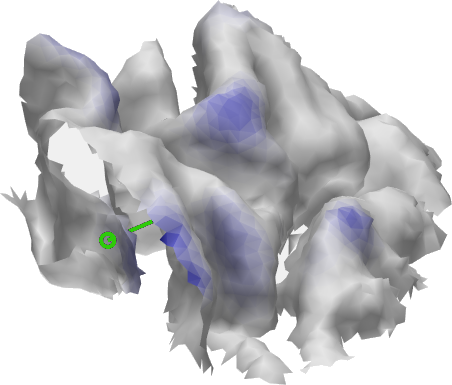
\includegraphics[height=2.0cm]{MEG_source_real_data.png} \\ MEG, clinical data
% \end{center}\end{minipage} \begin{minipage}{0.5cm} \begin{center}
% 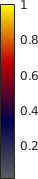
\includegraphics[height=2.5cm]{colorbar.png} \\ \null
% \end{center}
% \end{minipage} \vskip0.2cm
\end{center}
\end{footnotesize}
\caption{The placement and orientation of the synthetic source (green) in the 3b area in the posterior wall of the central sulcus. The image on the left shows the MAP reconstruction obtained with synthetic EEG data and on the right an almost identical reconstruction corresponding to the clinical data is shown.}
\label{fig:source_placement} 
\end{figure}

\begin{table}[h!]
\caption{The estimate type (MAP/CM), data modality (EEG/MEG), hyperprior (G/IG) and hyperparameter values for the different inverse estimates computed in this study. The scale parameter  value applied was, in general, smaller for EEG than for MEG. Again, restricting the computation in ROI allowed using a smaller scale parameter in CM computation than what was possible in MAP estimation. The shape parameter value 1.5 worked well in finding a MAP estimate. In the case of CM, a somewhat larger value was chosen in order to shorten the tail of the reconstruction and, thereby, to avoid overly focal reconstructions (Figure \ref{fig:gamma_vs_inverse_gamma}), which was necessary especially for IG}
\label{tab:inverse_estimates}
\centering
\begin{tabular}{|l|r|r|r|r|r|}
\hline
Type & Data & Res.\ & Hyperpr.\ & Shape &Scaling  \\
\hline
MAP & EEG & 1 mm & G & 1.5 & 1E-10   \\
 &  & 2 mm & G & 1.5 & 1E-10   \\ 
 &  & 1 mm & IG & 1.5 & 1E-10   \\
 &  & 2 mm & IG & 1.5 & 1E-10   \\ 
 MAP & MEG & 1 mm & G & 1.5 & 1E-5   \\
 &  & 2 mm & G & 1.5 & 1E-5   \\ 
 &  & 1 mm & IG & 1.5 & 1E-5   \\
 &  & 2 mm & IG & 1.5 & 1E-5   \\ 
 CM & EEG & 1 mm & G & 3 & 1E-12   \\
 &  & 2 mm & G & 3 & 1E-12   \\ 
 &  & 1 mm & IG & 50 & 1E-10   \\
 &  & 2 mm & IG & 3 & 1E-11   \\ 
CM & MEG & 1 mm & G & 3 & 1E-8   \\
 &  & 2 mm & G & 3 &  1E-10   \\ 
 &  & 1 mm & IG & 3 & 1E-8   \\
 &  & 2 mm & IG & 3 & 1E-10   \\ 
\hline
\end{tabular}
\end{table} 


\subsubsection{Implemetation with Zeffiro Interface}

\begin{figure}[h!]
\begin{footnotesize}
\begin{center}
\begin{minipage}{8.6cm} \begin{center}
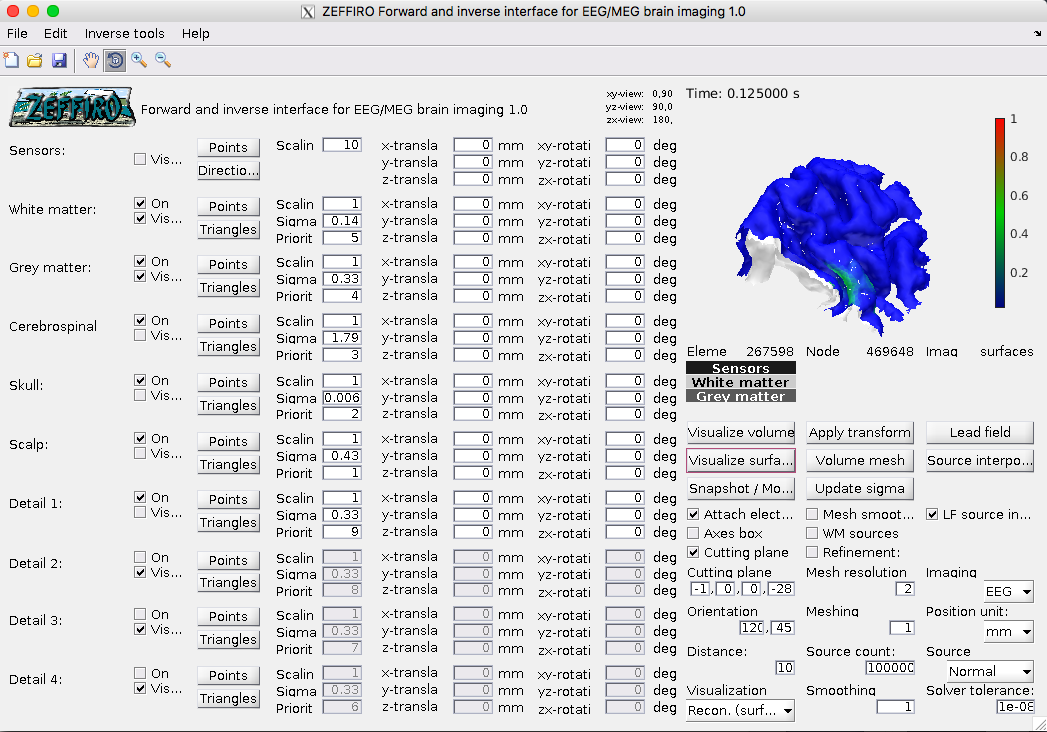
\includegraphics[width=8.6cm]{zeffiro_interface.png}
\end{center}
\end{minipage} 
\end{center}
\end{footnotesize}
\caption{{\em Zeffiro} Interface (I) \cite{ZeffiroInterface} is an open source code package for the Matlab (The MathWorks Inc.) environment, providing an easy-to-use tool for advanced multi-compartment finite element (FE) based EEG/MEG simulations. ZI is aimed to support studies which necessitate neurophysiologically accurate forward modeling, i.e., lead field matrix construction, source localization and time-lapse data analysis.}
\label{fig:zeffiro_interface} 
\end{figure}

The implementation of the present forward and inversion approaches is a part of the openly available Matlab (The MathWorks Inc.) based {\em Zeffiro}  Interface \cite{ZeffiroInterface} (ZI) which was developed during this study and was used as a platform for both forward and inverse computations. ZI  marks an open source based attempt to provide an easy-to-use tool for advanced finite element (FE) based EEG/MEG simulations. The name Zeffiro is Italian for 'a gentle breeze' referring to the simplicity and ease-of-use. ZI is aimed to support studies which necessitate neurophysiologically accurate forward modeling, i.e., lead field matrix construction, source localization and time-lapse data analysis. It is also designed to serve as a test platform for advanced inversion methods such as the hierarchical Bayesian approach. An important goal in the development of the ZI is also to motivate future directions on how the FEM can be effectively and conveniently applied in brain activity imaging and modulation interfaces. The main window of the ZI as it appears in the inversion computations is shown in Figure \ref{fig:zeffiro_interface}.

The volume mesh can be created via ZI with different resolutions (1 and 2 mm in the current study) which represents the tetrahedron's size and after that the lead field matrix will be calculated. To this end, based on EEG or MEG data, locations and orientations respect to sensors or magnetometers along with points and triangles for creating mesh will be imported individually. After creating the FE mesh it can be visualized from different angles. while conductivities for different tissue compartments have been defined. Alternatively, IAS MAP or MCMC estimation can be chosen for reconstruction of the source dipole and it can be visualized either from the surface segmentation or volumetric mesh. 

With ZI, one can segment a realistic multilayer geometry and generate a regular tetrahedral mesh, if triangular surface grids are available. In an up-to-date workstation, ZI allows for using a sub 1 mm modeling accuracy altogether for nine different conductivity compartments with reasonably short computation times.  Consequently, one can operate with a highly  realistic multi-compartment FE mesh.  

\subsubsection{GPU Capability} 

To tackle the issue of the computational cost, ZI utilizes a Graphics Processing Unit (GPU) in the following processes: (1)  segmenting the FE grid, (2) creating the lead field, (3)  source space interpolation, and (4) Inverting the data.  GPU is essentially an effective multi-processor parallel computing device which enables speeding up various tasks of scientific computing. Due  to the recent rapid development of GPUs, the parallel computing resources provided by a standard computer has tremendously increased. When evaluated in a GPU, an ordinary matrix-vector product can typically be computed in 1/100--1/10 of the time which would be taken by the Central Processing Unit (CPU) core for the same operation. Consequently, processing a high-definition finite element mesh and the corresponding matrices can be speed up significantly via employing a GPU instead of a CPU for the core procedures.  The ability to utilize the GPU is particularly important regarding the Matlab environment, which currently does not parallelize the sparse matrices resulting from the FE discretization in CPU. Therefore, a state-of-the-art GPU is practically necessary, if the goal is to produce a lead field for a physiologically accurate head model. 

The following reference computation times were obtained for 1 mm resolution 6-compartment test mesh with 36M elements, 6M nodes and ~0.5M sources using Lenovo P910 ThinkStation equipped with 2 x Intel Xeon E5-2697A v4 (RAM 256 GB) and 2 x NVIDIA Quadro P6000 (RAM 24 GB): (1) FE mesh generation: 1329 s, (2) EEG lead field for 128 electrodes: 2362 s, (3) MEG lead field for 154 magnetometers: 4826 s, (4) Source space interpolation: 212 s. Here the lead fields were tolerance refers to the 2-norm of the residual error.  

\section{Results}

\begin{figure}[h!]
\begin{footnotesize}
\begin{center}
\begin{minipage}{3cm} \begin{center}
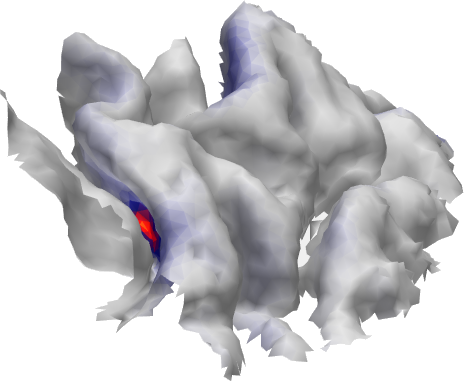
\includegraphics[height=2.0cm]{MAP_EEG_G_1mm.png} \\ EEG, 1 mm \\ Clinical data
\end{center}\end{minipage}
\begin{minipage}{3cm} \begin{center}
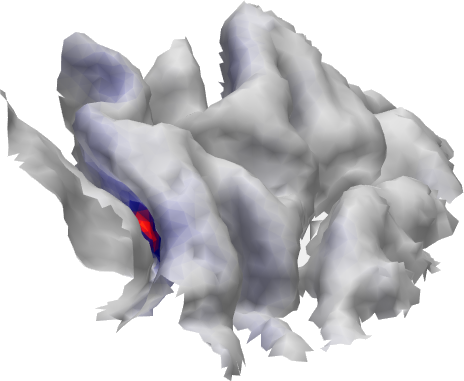
\includegraphics[height=2.0cm]{MAP_EEG_G_1mm_syntheticdata.png} \\ EEG, 1 mm \\ Synthetic data
\end{center}\end{minipage}\begin{minipage}{0.5cm} \begin{center}
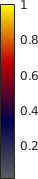
\includegraphics[height=2.5cm]{colorbar.png} \\ \mbox{}  \\ \mbox{}
\end{center}
\end{minipage} \vskip0.2cm
\begin{minipage}{3cm} \begin{center}
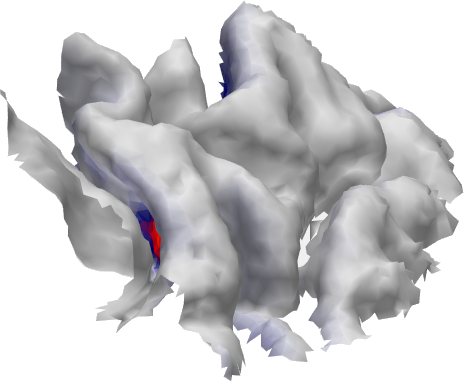
\includegraphics[height=2.0cm]{MAP_EEG_G_2mm.png}\\ EEG, 2 mm \\ Clinical data
\end{center}\end{minipage}
\begin{minipage}{3cm} \begin{center}
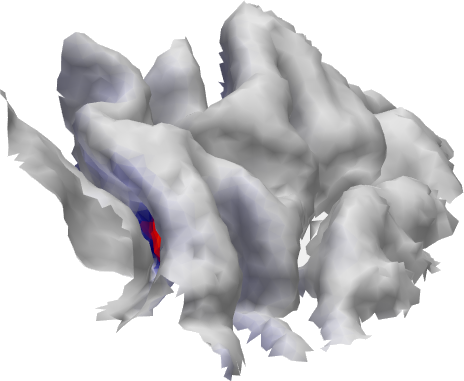
\includegraphics[height=2.0cm]{MAP_EEG_G_2mm_syntheticdata.png} \\ EEG, 2 mm \\ Synthetic data
\end{center}\end{minipage}
\begin{minipage}{0.5cm} \begin{center}
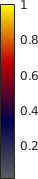
\includegraphics[height=2.5cm]{colorbar.png} \\ \mbox{} \\ \mbox{}
\end{center}
\end{minipage} \vskip0.2cm
\begin{minipage}{3cm} \begin{center}
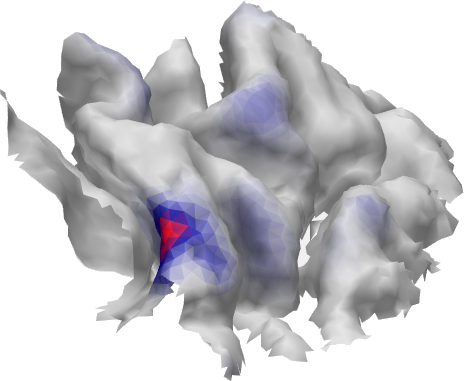
\includegraphics[height=2.0cm]{MAP_MEG_G_1mm.png} \\ MEG, 1 mm \\ Clinical data
\end{center}\end{minipage}
\begin{minipage}{3cm} \begin{center}
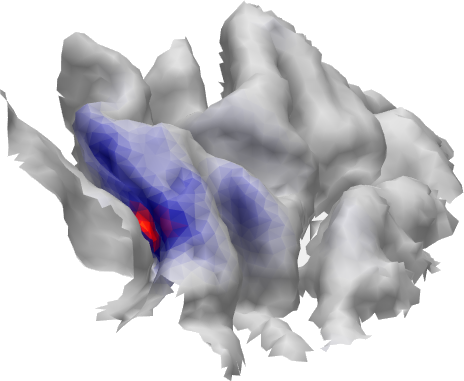
\includegraphics[height=2.0cm]{MAP_MEG_G_1mm_syntheticdata.png} \\ MEG, 1 mm \\ Synthetic data
\end{center}\end{minipage}\begin{minipage}{0.5cm} \begin{center}
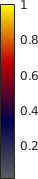
\includegraphics[height=2.5cm]{colorbar.png} \\ \mbox{} \\ \mbox{}
\end{center}
\end{minipage} \vskip0.2cm
\begin{minipage}{3cm} \begin{center}
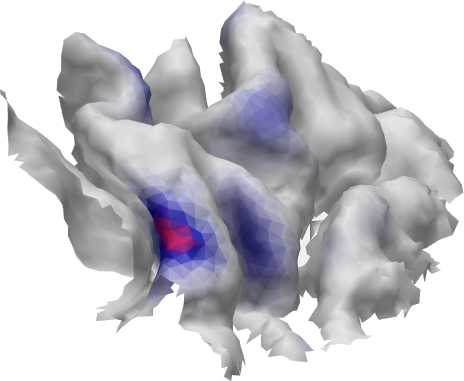
\includegraphics[height=2.0cm]{MAP_MEG_G_2mm.png}\\ MEG, 2 mm \\ Clinical data
\end{center}\end{minipage}
\begin{minipage}{3cm} \begin{center}
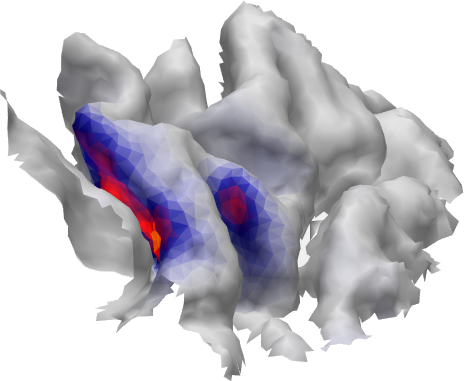
\includegraphics[height=2.0cm]{MAP_MEG_G_2mm_syntheticdata.png} \\ MEG, 2 mm \\ Synthetic data
\end{center}\end{minipage}
\begin{minipage}{0.5cm} \begin{center}
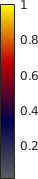
\includegraphics[height=2.5cm]{colorbar.png} \\ \mbox{} \\ \mbox{}
\end{center}
\end{minipage}
\end{center}
\end{footnotesize}
\caption{The MAP estimation results obtained with the IAS iteration and the gamma (G) hyperprior. The left column corresponds to real and the right one to synthetic data.}
\label{fig:somatosensory_results_1} 
\end{figure}

\begin{figure}[h!]
\begin{footnotesize}
\begin{center}
\begin{minipage}{3cm} \begin{center}
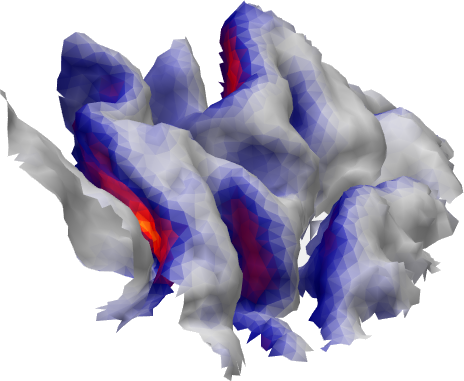
\includegraphics[height=2.0cm]{MAP_EEG_IG_1mm.png} \\ EEG, 1 mm \\ Clinical data
\end{center}\end{minipage}
\begin{minipage}{3cm} \begin{center}
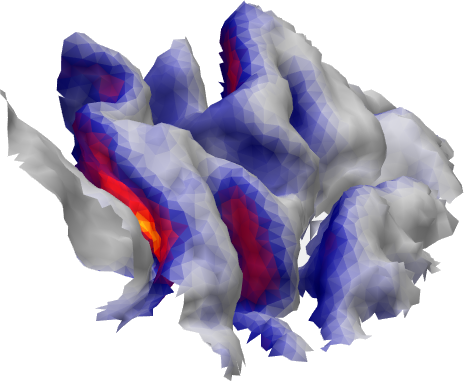
\includegraphics[height=2.0cm]{MAP_EEG_IG_1mm_syntheticdata.png} \\ EEG, 1 mm \\ Synthetic data
\end{center}\end{minipage}\begin{minipage}{0.5cm} \begin{center}
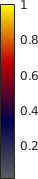
\includegraphics[height=2.5cm]{colorbar.png} \\ \mbox{}  \\ \mbox{}
\end{center}
\end{minipage} \vskip0.2cm
\begin{minipage}{3cm} \begin{center}
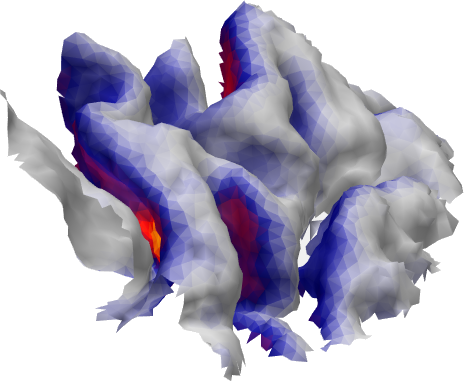
\includegraphics[height=2.0cm]{MAP_EEG_IG_2mm.png}\\ EEG, 2 mm \\ Clinical data
\end{center}\end{minipage}
\begin{minipage}{3cm} \begin{center}
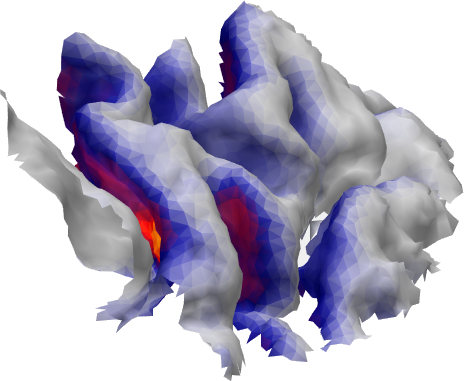
\includegraphics[height=2.0cm]{MAP_EEG_IG_2mm_syntheticdata.png} \\ EEG, 2 mm \\ Synthetic data
\end{center}\end{minipage}
\begin{minipage}{0.5cm} \begin{center}
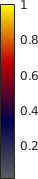
\includegraphics[height=2.5cm]{colorbar.png} \\ \mbox{} \\ \mbox{}
\end{center}
\end{minipage} \vskip0.2cm
\begin{minipage}{3cm} \begin{center}
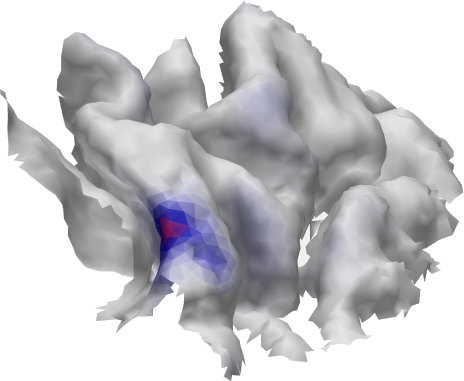
\includegraphics[height=2.0cm]{MAP_MEG_IG_1mm.png} \\ MEG, 1 mm \\ Clinical data
\end{center}\end{minipage}
\begin{minipage}{3cm} \begin{center}
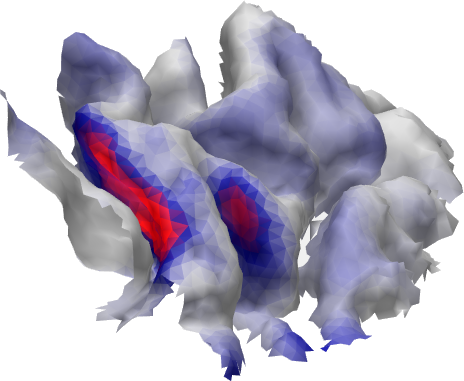
\includegraphics[height=2.0cm]{MAP_MEG_IG_1mm_syntheticdata.png} \\ MEG, 1 mm \\ Synthetic data
\end{center}\end{minipage}\begin{minipage}{0.5cm} \begin{center}
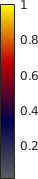
\includegraphics[height=2.5cm]{colorbar.png} \\ \mbox{} \\ \mbox{}
\end{center}
\end{minipage} \vskip0.2cm
\begin{minipage}{3cm} \begin{center}
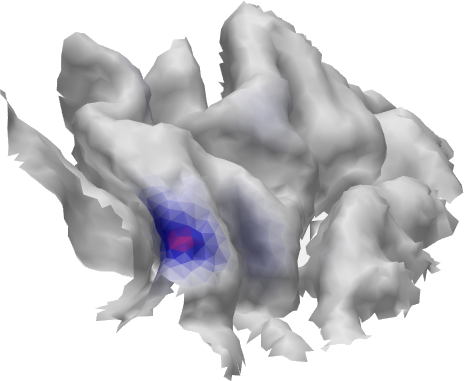
\includegraphics[height=2.0cm]{MAP_MEG_IG_2mm.png}\\ MEG, 2 mm \\ Clinical data
\end{center}\end{minipage}
\begin{minipage}{3cm} \begin{center}
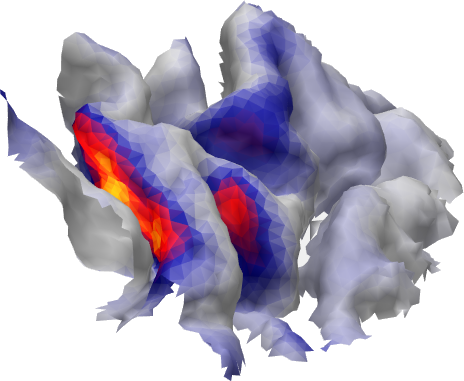
\includegraphics[height=2.0cm]{MAP_MEG_IG_2mm_syntheticdata.png} \\ MEG, 2 mm \\ Synthetic data
\end{center}\end{minipage}
\begin{minipage}{0.5cm} \begin{center}
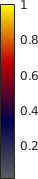
\includegraphics[height=2.5cm]{colorbar.png} \\ \mbox{} \\ \mbox{}
\end{center}
\end{minipage}
\end{center}
\end{footnotesize}
\caption{The MAP estimation results obtained with the IAS iteration and the inverse gamma (IG) hyperprior. The left column corresponds to real and the right one to synthetic data.}
\label{fig:somatosensory_results_1} 
\end{figure}


\begin{figure}[h!]
\begin{footnotesize}
\begin{center}
\begin{minipage}{3cm} \begin{center}
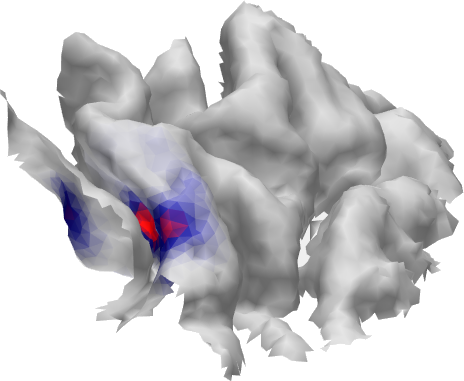
\includegraphics[height=2.0cm]{CM_EEG_G_1mm.png} \\ EEG, 1 mm \\ Clinical data
\end{center}\end{minipage}
\begin{minipage}{3cm} \begin{center}
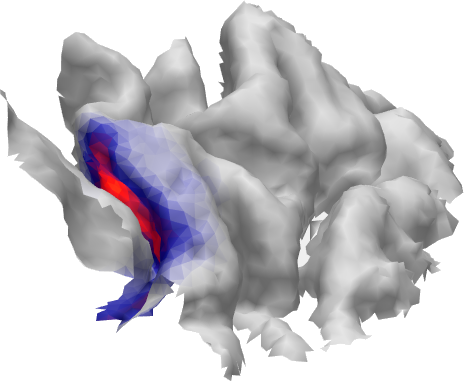
\includegraphics[height=2.0cm]{CM_EEG_G_1mm_syntheticdata.png} \\ EEG, 1 mm \\ Synthetic data
\end{center}\end{minipage} \begin{minipage}{0.5cm} \begin{center}
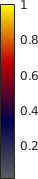
\includegraphics[height=2.5cm]{colorbar.png} \\ \mbox{} \\ \mbox{}
\end{center}
\end{minipage} \vskip0.2cm
\begin{minipage}{3cm} \begin{center}
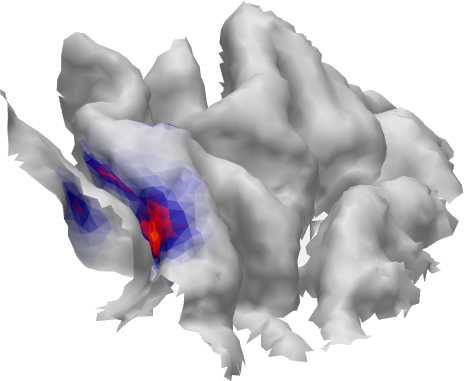
\includegraphics[height=2.0cm]{CM_EEG_G_2mm.png}\\ EEG, 2 mm \\ Clinical data
\end{center}\end{minipage}
\begin{minipage}{3cm} \begin{center}
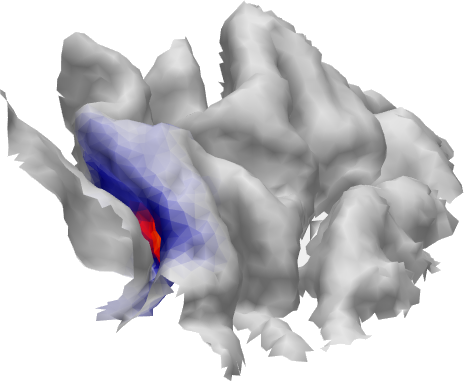
\includegraphics[height=2.0cm]{CM_EEG_G_2mm_syntheticdata.png} \\ EEG, 2 mm \\ Synthetic data
\end{center}\end{minipage}
\begin{minipage}{0.5cm} \begin{center}
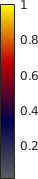
\includegraphics[height=2.5cm]{colorbar.png} \\ \mbox{} \\ \mbox{}
\end{center}
\end{minipage} \vskip0.2cm
\begin{minipage}{3cm} \begin{center}
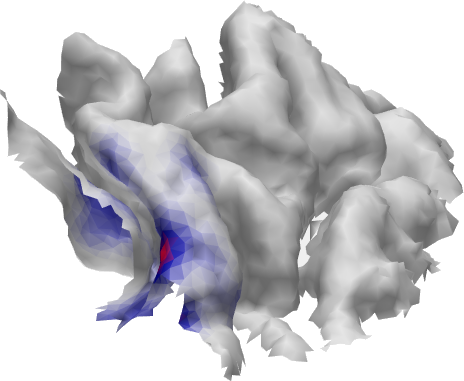
\includegraphics[height=2.0cm]{CM_MEG_G_1mm.png} \\ MEG, 1 mm \\ Clinical data
\end{center}\end{minipage}
\begin{minipage}{3cm} \begin{center}
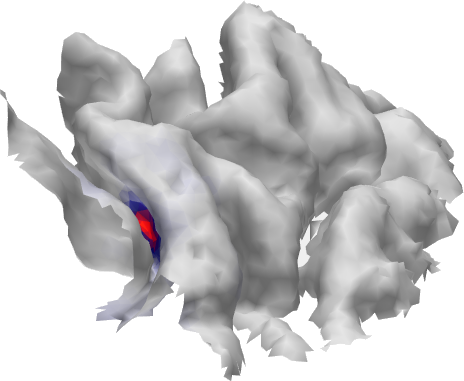
\includegraphics[height=2.0cm]{CM_MEG_G_1mm_syntheticdata.png} \\ MEG, 1 mm \\ Synthetic data
\end{center}\end{minipage} \begin{minipage}{0.5cm} \begin{center}
\includegraphics[height=2.5cm]{colorbar.png} \\ \null
\end{center}
\end{minipage} \vskip0.2cm
\begin{minipage}{3cm} \begin{center}
\includegraphics[height=2.0cm]{CM_MEG_G_2mm.png}\\ MEG, 2 mm \\ Clinical data 
\end{center}\end{minipage}
\begin{minipage}{3cm} \begin{center}
\includegraphics[height=2.0cm]{CM_MEG_G_2mm_syntheticdata.png} \\ MEG, 2 mm \\ Synthetic data
\end{center}\end{minipage}
\begin{minipage}{0.5cm} \begin{center}
\includegraphics[height=2.5cm]{colorbar.png} \\ \mbox{} \\ \mbox{}
\end{center}
\end{minipage}
\end{center}
\end{footnotesize}
\caption{The CM estimation results obtained with the Gibbs sampler and the gamma (G) hyperprior. The left column corresponds to real and the right one to synthetic data.}
\label{fig:somatosensory_results_2} 
\end{figure}


\begin{figure}[h!]
\begin{footnotesize}
\begin{center}
\begin{minipage}{3cm} \begin{center}
\includegraphics[height=2.0cm]{CM_EEG_IG_1mm.png} \\ EEG, 1 mm \\ Clinical data
\end{center}\end{minipage}
\begin{minipage}{3cm} \begin{center}
\includegraphics[height=2.0cm]{CM_EEG_IG_1mm_syntheticdata.png} \\ EEG, 1 mm \\ Synthetic data
\end{center}\end{minipage} \begin{minipage}{0.5cm} \begin{center}
\includegraphics[height=2.5cm]{colorbar.png} \\ \mbox{} \\ \mbox{}
\end{center}
\end{minipage} \vskip0.2cm
\begin{minipage}{3cm} \begin{center}
\includegraphics[height=2.0cm]{CM_EEG_IG_2mm.png}\\ EEG, 2 mm \\ Clinical data
\end{center}\end{minipage}
\begin{minipage}{3cm} \begin{center}
\includegraphics[height=2.0cm]{CM_EEG_IG_2mm_syntheticdata.png} \\ EEG, 2 mm \\ Synthetic data
\end{center}\end{minipage}
\begin{minipage}{0.5cm} \begin{center}
\includegraphics[height=2.5cm]{colorbar.png} \\ \mbox{} \\ \mbox{}
\end{center}
\end{minipage} \vskip0.2cm
\begin{minipage}{3cm} \begin{center}
\includegraphics[height=2.0cm]{CM_MEG_IG_1mm.png} \\ MEG, 1 mm \\ Clinical data
\end{center}\end{minipage}
\begin{minipage}{3cm} \begin{center}
\includegraphics[height=2.0cm]{CM_MEG_IG_1mm_syntheticdata.png} \\ MEG, 1 mm \\ Synthetic data
\end{center}\end{minipage} \begin{minipage}{0.5cm} \begin{center}
\includegraphics[height=2.5cm]{colorbar.png} \\ \null
\end{center}
\end{minipage} \vskip0.2cm
\begin{minipage}{3cm} \begin{center}
\includegraphics[height=2.0cm]{CM_MEG_IG_2mm.png}\\ MEG, 2 mm \\ Clinical data 
\end{center}\end{minipage}
\begin{minipage}{3cm} \begin{center}
\includegraphics[height=2.0cm]{CM_MEG_IG_2mm_syntheticdata.png} \\ MEG, 2 mm \\ Synthetic data
\end{center}\end{minipage}
\begin{minipage}{0.5cm} \begin{center}
\includegraphics[height=2.5cm]{colorbar.png} \\ \mbox{} \\ \mbox{}
\end{center}
\end{minipage}
\end{center}
\end{footnotesize}
\caption{The CM estimation results obtained with the Gibbs sampler and the inverse gamma (IG) hyperprior. The left column corresponds to real and the right one to synthetic data.}
\label{fig:somatosensory_results_2} 
\end{figure}

The results are included in Figures \ref{fig:somatosensory_results_1}, \ref{fig:source_placement} and \ref{fig:somatosensory_results_2} which visualize the reconstructed activity on the grey matter surface near the left primary somatosensory cortex in the direction of the inward surface normal. The hierarchical Bayesian approach was found to produce focal reconstructions in which the maximum was localized near area 3b of the N20 component. 

\subsection{MAP estimation}

In IAS MAP estimation, most notably, EEG was observed to localize the activity deeper than MEG. For EEG, the sulcus wall is clearly active in each reconstruction. The estimates obtained with the G hyperprior are significantly more focal than those produced using IG. In the EEG 
reconstructions, the activity is mainly distributed on sulcus. 
The results obtained with the synthetic dipolar source were qualitatively similar to the case of the clinical data, suggesting that the real activity is at area 3b. 

For MEG, the position of the activity corresponded well with the EEG reconstructions in a global scale. However, locally it was more superficial being supported rather on the gyrus than on sulcus. A focal reconstruction concentrated on the same area was found using both G and IG hyperprior. The comparison between the real and synthetic data revealed more differences for MEG than what was found for EEG, as the deeper sulcal activity was clearly reconstructed only for synthetic data in the case of MEG. 

\subsection{CM estimation}

The CM estimates obtained with the Gibbs sampler were, in general, more focal than what was obtained with the IAS algorithm, especially, for localizing deeper sources. For EEG, the CM estimate for the activity corresponded mainly with the MAP results, as the main activity was concentrated on the same area of the sulcus wall. Notably, the MEG estimates obtained with the IG hyperprior matched well with these results. 

Compared to the G hyperprior, IG  produced, overall, more focal results and an enhanced placement of the reconstructed activity. IG localized the activity to the the close proximity the synthetic source position for each source in each test case.  Adjusting the shape and scale parameter for IG required more tuning than for G, to avoid overly focal estimates and also to help the sampler to find the essential part of the posterior distribution. 

%Sampsa,eikö se parempi että laittamme MAP & CM kuvat vieressä? esim, Kuva 9 voi olla MAP (G) hyperprior.


\subsubsection{FE mesh}

The FE mesh resolution effect was observed to have a minor effect on the reconstruction process. Differences between 1 and 2 mm resolution were observed mainly for the focal MAP reconstructions for which the maximum of the detected activity distribution has up to 5-7 mm difference in distance.  Of these, the ones obtained with the 1 mm mesh matched better with the synthetic source position which was particularly obvious in the case of EEG. For CM, such differences were not observed. 

\section{Discussion}

The results of this study suggest that the  present hierarchical Bayesian approach for reconstructing the primary current distribution of the brain  \citep{calvetti2009, lucka2012} can be advantageous in  reconstructing evoked N20 activity, in particular, if an accurate MRI-based multi-compartment head segmentation is available. Based on the present results, it seems that by estimating a hierarchical posterior distribution a source localization accuracy of 5 mm or better can be achieved, if a 1 mm FE mesh resolution is used. It was also observed that obtaining the best possible accuracy may necessitate estimating the CM via the Gibbs sampling approach and defining a ROI for the sampler.  Due to this finding and the fact that the present IAS MAP estimation technique can be associated with the minimum current and minimum support estimate (MCE and MSE) \cite{uutela1999visualization,nagarajan2006controlled}
primary current density, it also seems that the hierarchical Bayesian model can match or even outperform many classical iterative regularization techniques with respect to the source localization accuracy. 

Here, the evoked activity was successfully found as an intensity distribution which is classically known to be challenging, especially, concerning sulcal activity, such as N20 which is associated with the Brodmann area 3b in the posterior wall of the central sulcus. %The hierarchical Bayesian probability model was observed to be a crucial part of source localization process.  %Namely, with respect to MAP estimation, it can be associated with the classical MCE and MSE optimization techniques, but it also allows finding an enhanced reconstruction via estimating the CM. 
% \textcolor{red}{Since the inverse problem of E/MEG is an ill-posed approach it provides non-uniqueness solution of current source distribution due to not configuring all the sources on the scalp. Therefore, Minimum Current Estimate considered as source localization technique even in the areas with less activity by minimizing the {\em $\ell^1$}-norm \cite{matsuura1995selective} which can converge to the global solution by linear programming and is more focal than Euclidean {\em $\ell^2$}-norm and recognize and measure sources in sensory areas. In maximum a posterior probability of hierarchical Bayesian, minimum {\em $l^{2}$} considers Gaussian a prior current distribution and {\em $l^{1}$} considers an exponential a prior current distribution 
% \cite{uutela1999visualization,stenbacka2002comparison}. }
An estimate of the CM was found to be generally more robust than a MAP-based reconstruction. Finding a CM estimate was vital when inverting MEG data, if the goal is to localize reconstructed distribution in the sulcus wall, instead of detecting it indirectly based on tangential activity on the gyral part. These observations are in agreement with the general {\em knowledge} of E/MEG according to which EEG is {\em per se} sensitive to deeper activity than MEG \citep{hari2018ifcn,hari1990neuromagnetic} but that MEG sees also those parts \citep{attal2009,coffey2016cortical}. 

The present results suggest that the FE mesh resolution affected the inverse estimates and that the best localization accuracy was achieved with the 1 mm mesh regarding both MAP and CM. Using the 2 mm resolution led to around 5 mm localization differences between the cases of the actual and synthetic data. Notably, with the 1 mm resolution, the differences were optimally less than 5 mm, suggesting that the maximal spatial accuracy of the MEG (2-4 mm for superficial areas) \citep{tarkiainen20033d} was achieved, and that of the EEG was even surpassed \cite{cuffin2001realistically,cuffin2001spherical,grover2016fundamental,wang2009relationship}. Furthermore, it appears that the FE mesh resolution  specifically affects the EEG reconstruction accuracy, since the electric potential depends more strongly on the conductivity distribution than on the magnetic field \citep{hamalainen1993}. 

Akin to the findings of \cite{calvetti2009}, the most focal MAP and CM estimates were obtained using the gamma (G) and inverse gamma (IG) hyperprior, respectively. Moreover, IG was found to localize the activity deeper in CM estimation than G. These characteristics obviously follow from the long tail of the IG which emphasizes focal reconstructions. A posterior corresponding to a long-tailed hyperprior can be difficult to be maximized, since the maximum can be supported in a very small set. Therefore, on one hand, the  IAS MAP estimation algorithm yields a more robust outcome for G, which has a  shorter tail than IG. On the other hand, IG is advantageous in CM estimation, since the Gibbs sampler performs well even with very focally supported posterior densities, in particular, since here the sampling process is restricted to the ROI, i.e., a 24 mm diameter ball;  considering the restricted 24 mm diameter ball as target area to detect the exact activity of Somatosensory area in sulcus region, particularly for deeper source,i.e, in EEG \cite{hari2018ifcn}. % we know beforehand from the literature that somatosensory area is allocated in 3b area of the broadmann area which the location is in sulcus and therefore ,considering 24 diameters to restrict the activity in deep sulcus of 3b area.
Yet, in some cases, some tuning of the hyperparameters was needed for IG in order to make the sampler find the activity. Consequently, a deeper investigation of the hyperparameter selection would  be an important topic for the future research.

The present forward simulation approach was found to perform adequately with both 1 and 2 mm resolution. Agreeing with the existing knowledge on physiologically accurate volumetric head modeling and forward simulation \cite{demunck2012,rullmann2009eeg,wolters2007geometry}, the FE mesh resolution of 1 mm was found to be advantageous for optimizing the reconstruction quality.  The present GPU-based approach to the forward simulation was found to be essential in order to achieve a feasibly short computation times for mesh segmentation and lead field matrix evaluation using the {\em Zeffiro interface} \cite{ZeffiroInterface}, i.e., an opens source Matlab code package. Further ways to improve the existing forward solver might include using the neurophysiological normal constraint   in the inverse computation stage, or investigating the effect of the surface segmentation on the inversion outcome. In this study, the normal constraint was applied after inverting the data for a set of Cartesian source orientations. Based on our preliminary tests, taking into  account the actual (basically normal) orientation of the pyramidal cells in the forward simulation necessitates careful modeling, since the complex structure of the brain does not always allow determining the normal of the grey matter uniquely, and also since erroneous orientations are easily reflected as artifacts in the reconstructions. Furthermore, as the present surface segmentation was a preprocessed one, it would be important to explore the performance of the present FE mesh generation approach and its effect on inversion with a less optimal set of surfaces.

In future work, it will be necessary to apply the present inversion approach for more data sets, in order to learn more about the practical localization capability of the IAS algorithm and the Gibbs sampler, as in this study the sulcal activity  was detected with IAS for the  synthetic source but not when using clinical data. An inherent part of further comparisons will be depth-localization improving priors which can be based on physiological knowledge as proposed in  \cite{calvetti2015,calvetti2018}.  Also, an interesting future work direction would be to implement and study more inversion approaches using the existing open source interface. For example, a single-dipole reconstruction strategy, which is often utilized in localizing sulcal activity, could be considered as a topic.

\section*{Acknowledgments}

AR, QH, and SP were supported by the Academy of Finland Centre of Excellence in Inverse Modelling and Imaging 2018--2025. AK was supported by the Academy of Finland Postdoctoral Researcher grant number  316542.


\bibliographystyle{model1-num-names}
\bibliography{paper_ref.bib}

%% Authors are advised to submit their bibtex database files. They are
%% requested to list a bibtex style file in the manuscript if they do
%% not want to use model1-num-names.bst.

%% References without bibTeX database:

% \begin{thebibliography}{00}

%% \bibitem must have the following form:
%%   \bibitem{key}...
%%

% \bibitem{}

% \end{thebibliography}


\end{document}

%%
%% End of file `elsarticle-template-1-num.tex'.